\section*{Parallelization Steps}
\begin{description}
    \item[Sequential Program]Sequential Steps + Programming (Application specification $\rightarrow$ executable program)
    \item[Parallel Program]Parallelization + Programming. \\ %Analysis of seq. problems or programs to identify parallelism. \\
        % 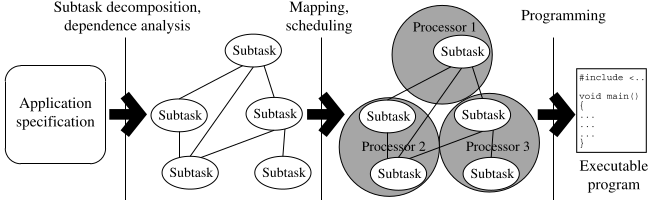
\includegraphics[width=0.4\linewidth]{paralellization.png} %TODO: modify image to include TLB
        \item[Decomposition] of apps into functional tasks / data blocks. (expose inherent concurrency). Influencing Factors:
        \begin{itemize}
            \item \textbf{Application Type}: distinct steps or iterative block of computations (task parallel, data parallel) %TODO: task parallel und data parallel erklären
            \item \textbf{Concurrency degree (max, avg)}: depending of degree of inherent parallelism. all/enough or none can be executed concurrently.
            \item \textbf{Granularity}: computational size of tasks / data blocks after decomposition. (fine, medium, coarse)
            \item \textbf{Target system}: affects costs of synchronization and communication. (\textit{Shared-mem arch}: support fine-grain decomp. inexpensive more frequent s \& c, \textit{Distr. mem arch}: usually require coarse-grain decomp. more expensive and less frequent.)
            %TODO: S. 19 - 23 Decomposition types
        \end{itemize}
    \item[Dependence Analysis]is critical to identify how much parallelism exists \& how it can be exploited.
            of \textbf{Control Dependencies} and \textbf{Data Dependencies}
        \item[Mapping] (assignment, part of scheduling) the exectuion of tasks / operations on data onto computing system.
        \item[Programming] or expressing parallelism in programming language.
        \item[] Note: Performance now a programmers charge. (cannot rely on HW anymore).
\end{description}
\section*{OpenMP}
